\documentclass[]{article}
\usepackage{lmodern}
\usepackage{amssymb,amsmath}
\usepackage{ifxetex,ifluatex}
\usepackage{fixltx2e} % provides \textsubscript
\ifnum 0\ifxetex 1\fi\ifluatex 1\fi=0 % if pdftex
  \usepackage[T1]{fontenc}
  \usepackage[utf8]{inputenc}
\else % if luatex or xelatex
  \ifxetex
    \usepackage{mathspec}
  \else
    \usepackage{fontspec}
  \fi
  \defaultfontfeatures{Ligatures=TeX,Scale=MatchLowercase}
\fi
% use upquote if available, for straight quotes in verbatim environments
\IfFileExists{upquote.sty}{\usepackage{upquote}}{}
% use microtype if available
\IfFileExists{microtype.sty}{%
\usepackage{microtype}
\UseMicrotypeSet[protrusion]{basicmath} % disable protrusion for tt fonts
}{}
\usepackage[margin=1in]{geometry}
\usepackage{hyperref}
\hypersetup{unicode=true,
            pdftitle={PM 1},
            pdfauthor={Felipe Domínguez},
            pdfborder={0 0 0},
            breaklinks=true}
\urlstyle{same}  % don't use monospace font for urls
\usepackage{graphicx,grffile}
\makeatletter
\def\maxwidth{\ifdim\Gin@nat@width>\linewidth\linewidth\else\Gin@nat@width\fi}
\def\maxheight{\ifdim\Gin@nat@height>\textheight\textheight\else\Gin@nat@height\fi}
\makeatother
% Scale images if necessary, so that they will not overflow the page
% margins by default, and it is still possible to overwrite the defaults
% using explicit options in \includegraphics[width, height, ...]{}
\setkeys{Gin}{width=\maxwidth,height=\maxheight,keepaspectratio}
\IfFileExists{parskip.sty}{%
\usepackage{parskip}
}{% else
\setlength{\parindent}{0pt}
\setlength{\parskip}{6pt plus 2pt minus 1pt}
}
\setlength{\emergencystretch}{3em}  % prevent overfull lines
\providecommand{\tightlist}{%
  \setlength{\itemsep}{0pt}\setlength{\parskip}{0pt}}
\setcounter{secnumdepth}{0}
% Redefines (sub)paragraphs to behave more like sections
\ifx\paragraph\undefined\else
\let\oldparagraph\paragraph
\renewcommand{\paragraph}[1]{\oldparagraph{#1}\mbox{}}
\fi
\ifx\subparagraph\undefined\else
\let\oldsubparagraph\subparagraph
\renewcommand{\subparagraph}[1]{\oldsubparagraph{#1}\mbox{}}
\fi

%%% Use protect on footnotes to avoid problems with footnotes in titles
\let\rmarkdownfootnote\footnote%
\def\footnote{\protect\rmarkdownfootnote}

%%% Change title format to be more compact
\usepackage{titling}

% Create subtitle command for use in maketitle
\newcommand{\subtitle}[1]{
  \posttitle{
    \begin{center}\large#1\end{center}
    }
}

\setlength{\droptitle}{-2em}

  \title{PM 1}
    \pretitle{\vspace{\droptitle}\centering\huge}
  \posttitle{\par}
    \author{Felipe Domínguez}
    \preauthor{\centering\large\emph}
  \postauthor{\par}
    \date{}
    \predate{}\postdate{}
  

\begin{document}
\maketitle

\subparagraph{Semana 16/08 - 30/08}\label{semana-1608---3008}

\begin{center}\rule{0.5\linewidth}{\linethickness}\end{center}

Objetivos de la semana:

\begin{itemize}
\item
  Graficar:

  \begin{itemize}
  \tightlist
  \item
    Cantidad de alumnos que toman los distintos exploratorios\\
  \item
    Cantidad de exploratorios que toman los alumnos.
  \end{itemize}
\end{itemize}

\newline

\begin{itemize}
\item
  Profundizar en la hipotesis H3: Depende de trayectorias educacionales
  (TE) que muestran desorientación.

  \begin{itemize}
  \tightlist
  \item
    H3.1: depende de TE que incluyen varios cursos exploratorios\\
  \item
    H3.2: depende de TE que incluyen cursos de varios majors/minors
  \end{itemize}
\end{itemize}

\begin{center}\rule{0.5\linewidth}{\linethickness}\end{center}

\newline

\subparagraph{Importamos los datos y imprimimos el
header}\label{importamos-los-datos-y-imprimimos-el-header}

Fueron importatos los datos de cada año por separado, y además se juntó
la información de las 4 generaciones.

\begin{verbatim}
##  [1] "X"                         "RUT"                      
##  [3] "N_ALUMNO"                  "ANO_ADMISION"             
##  [5] "PROGRAMA_CODIGO"           "PROGRAMA"                 
##  [7] "MAJOR_CODIGO_SELECCIONADO" "MAJOR_SELECCIONADO"       
##  [9] "MAJOR_TRACK.AREA"          "MINOR_CODIGO_SELECCIONADO"
## [11] "MINOR_SELECCIONADO"        "CREDITOS_ALUMNO"          
## [13] "CURSO_CURRICULUM"          "CURSO_PROGRAMA"           
## [15] "ANO"                       "SEMESTRE"                 
## [17] "SIGLA"                     "SECCION"                  
## [19] "NOMBRE_CURSO"              "CREDITOS_CURSO"           
## [21] "NOTA_FINAL"                "NOTA_FINAL_ALFA"          
## [23] "PPA_Global"                "Estado_en_DARA"           
## [25] "VIA_INGRESO"               "VIA_CASO_INGRESO"
\end{verbatim}

\newline

Para este primer análisis, es necesario listar los distintos
exploratorios que ofrecen los majors. Los datos fueron sacados de la
página del Siding.

\newline
\newline
\newline

\begin{center}\rule{0.5\linewidth}{\linethickness}\end{center}

\paragraph{Cantidad de alumnos que toman los distintos
exploratorios}\label{cantidad-de-alumnos-que-toman-los-distintos-exploratorios}

\begin{center}\rule{0.5\linewidth}{\linethickness}\end{center}

\begin{center}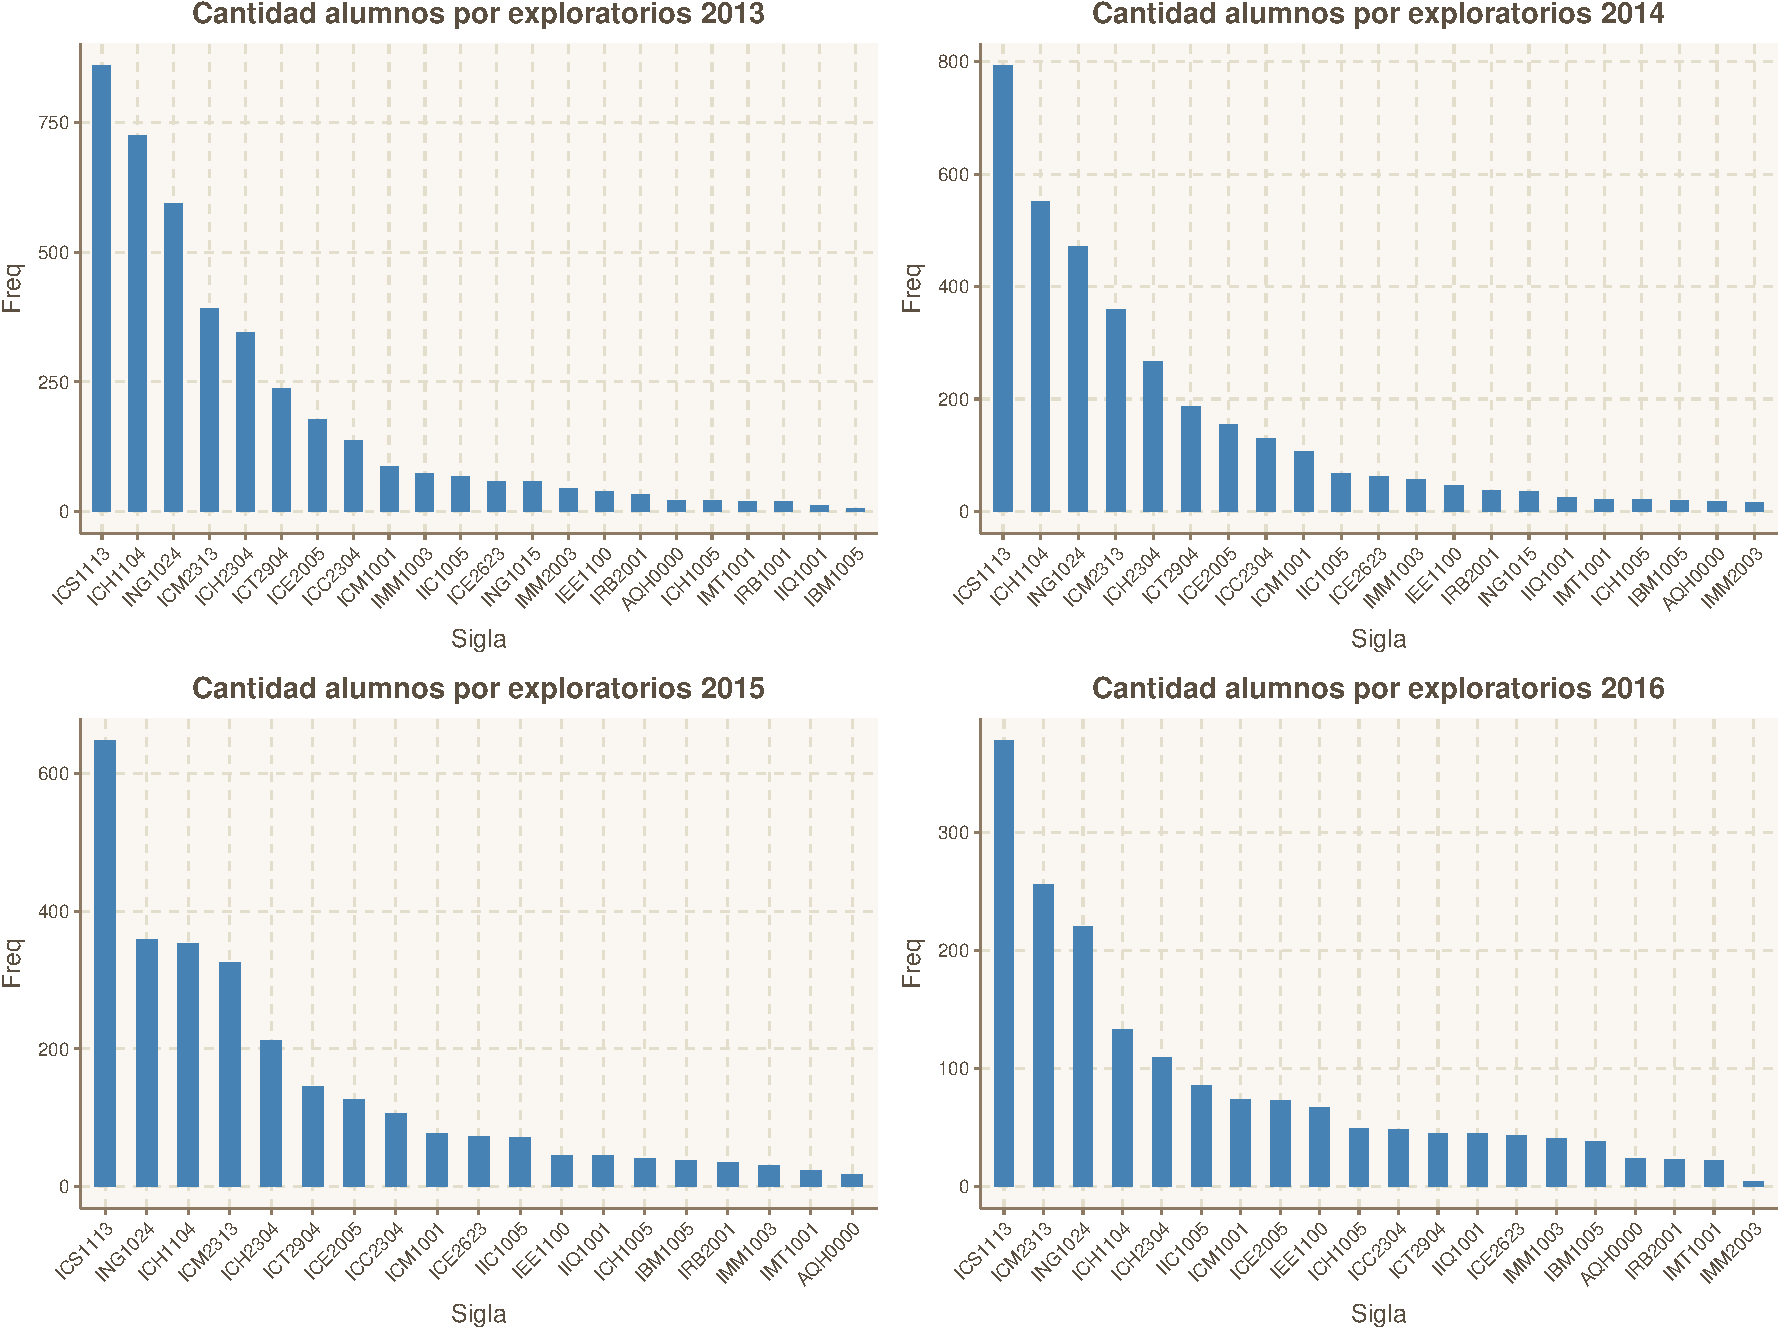
\includegraphics{Figs/plot-1} 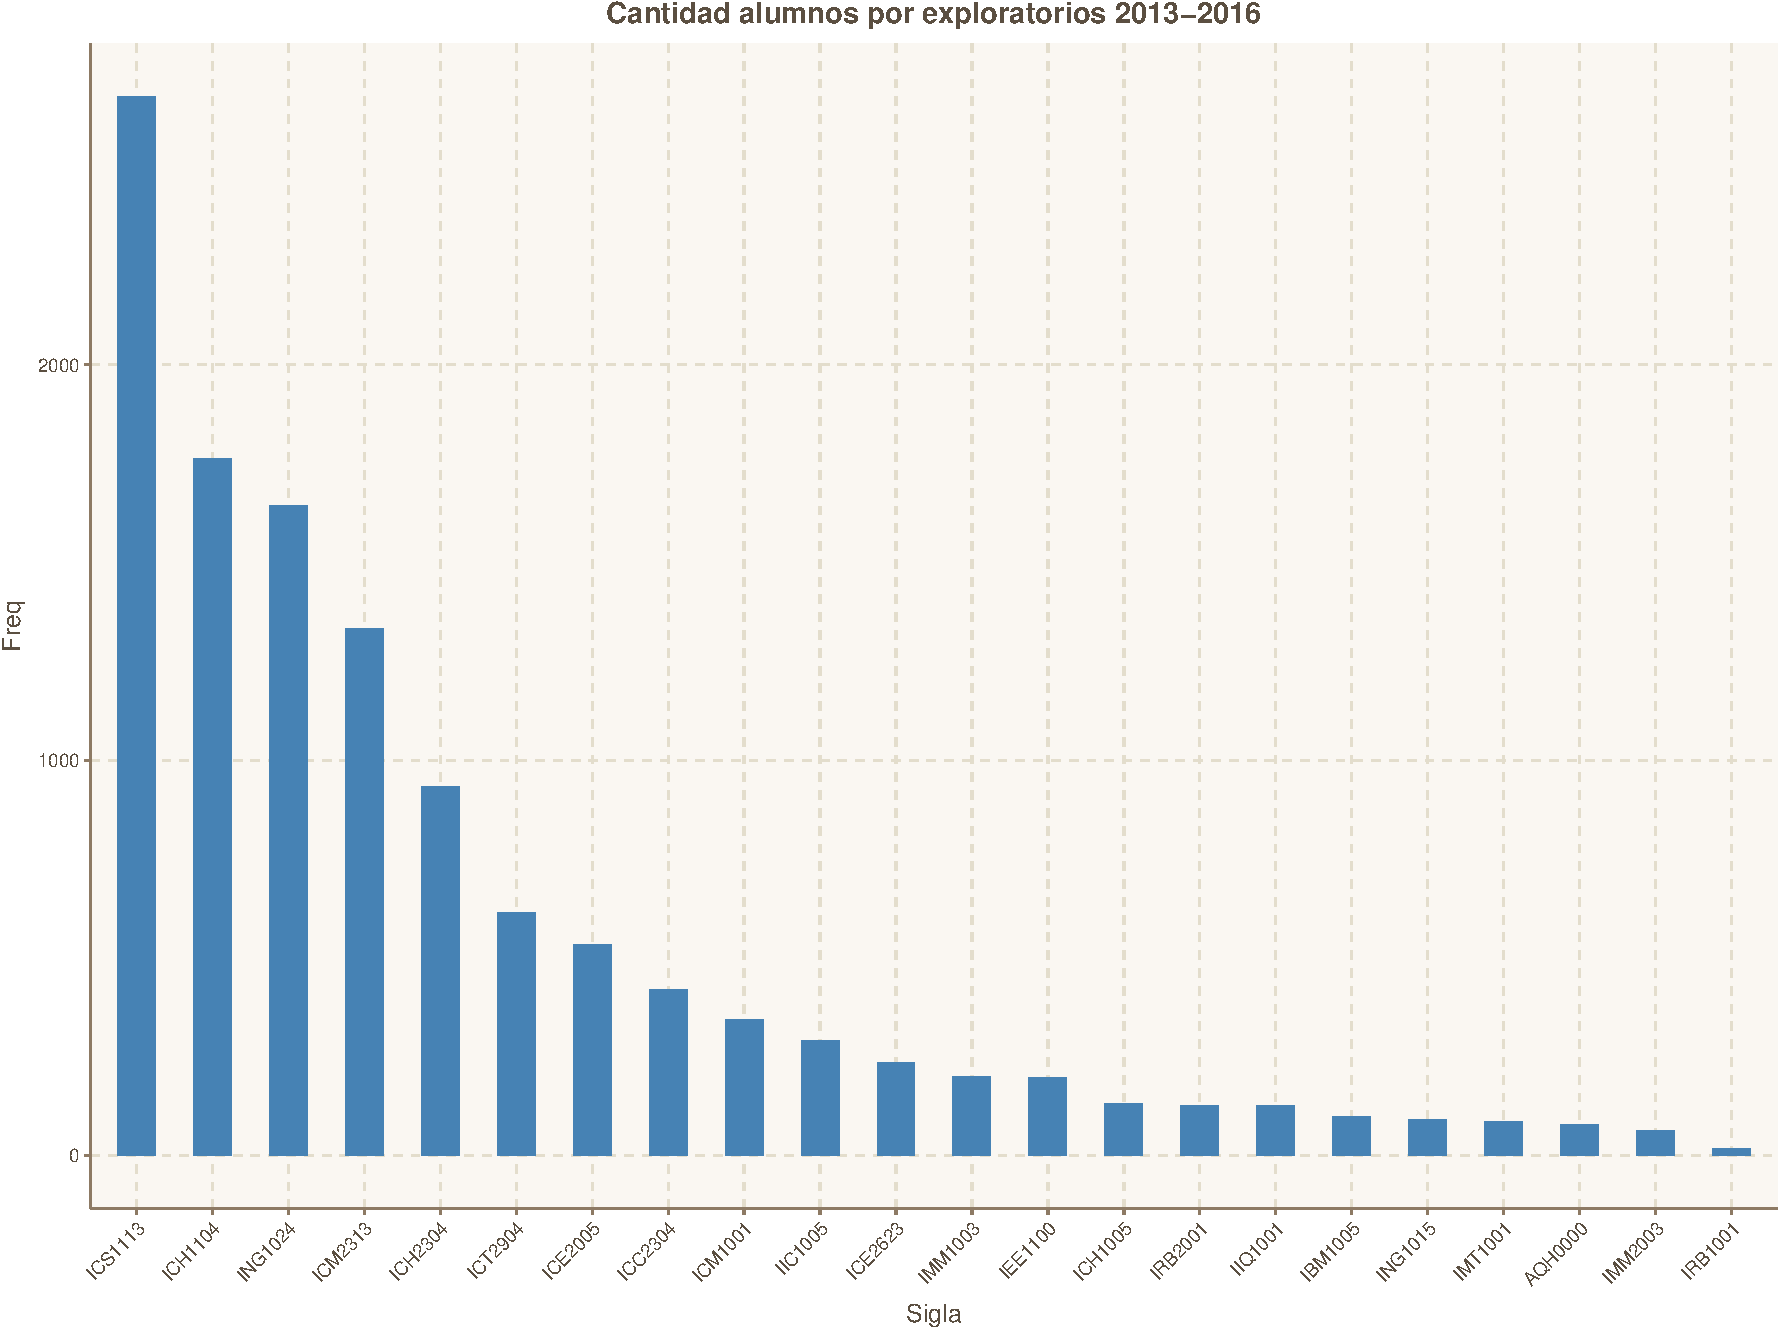
\includegraphics{Figs/plot-2} \end{center}

En el gráfico 1, podemos ver que los 3 eploratorios más tomados
corresponden a:

\begin{itemize}
\tightlist
\item
  Optimización (ICS1113)\\
\item
  Mecánica de Fluidos (ICH1104)\\
\item
  ING(1024)
\end{itemize}

Pero estos cursos corresponden a cursos mínimos de las especializades
más tomadas, por lo tanto es necesario filtrar los datos para no incluir
ramos de la especialidad de cada alumno.

\newline   \newline

\begin{center}\rule{0.5\linewidth}{\linethickness}\end{center}

\paragraph{Cantidad de exploratorios
tomados}\label{cantidad-de-exploratorios-tomados}

\begin{center}\rule{0.5\linewidth}{\linethickness}\end{center}

\begin{center}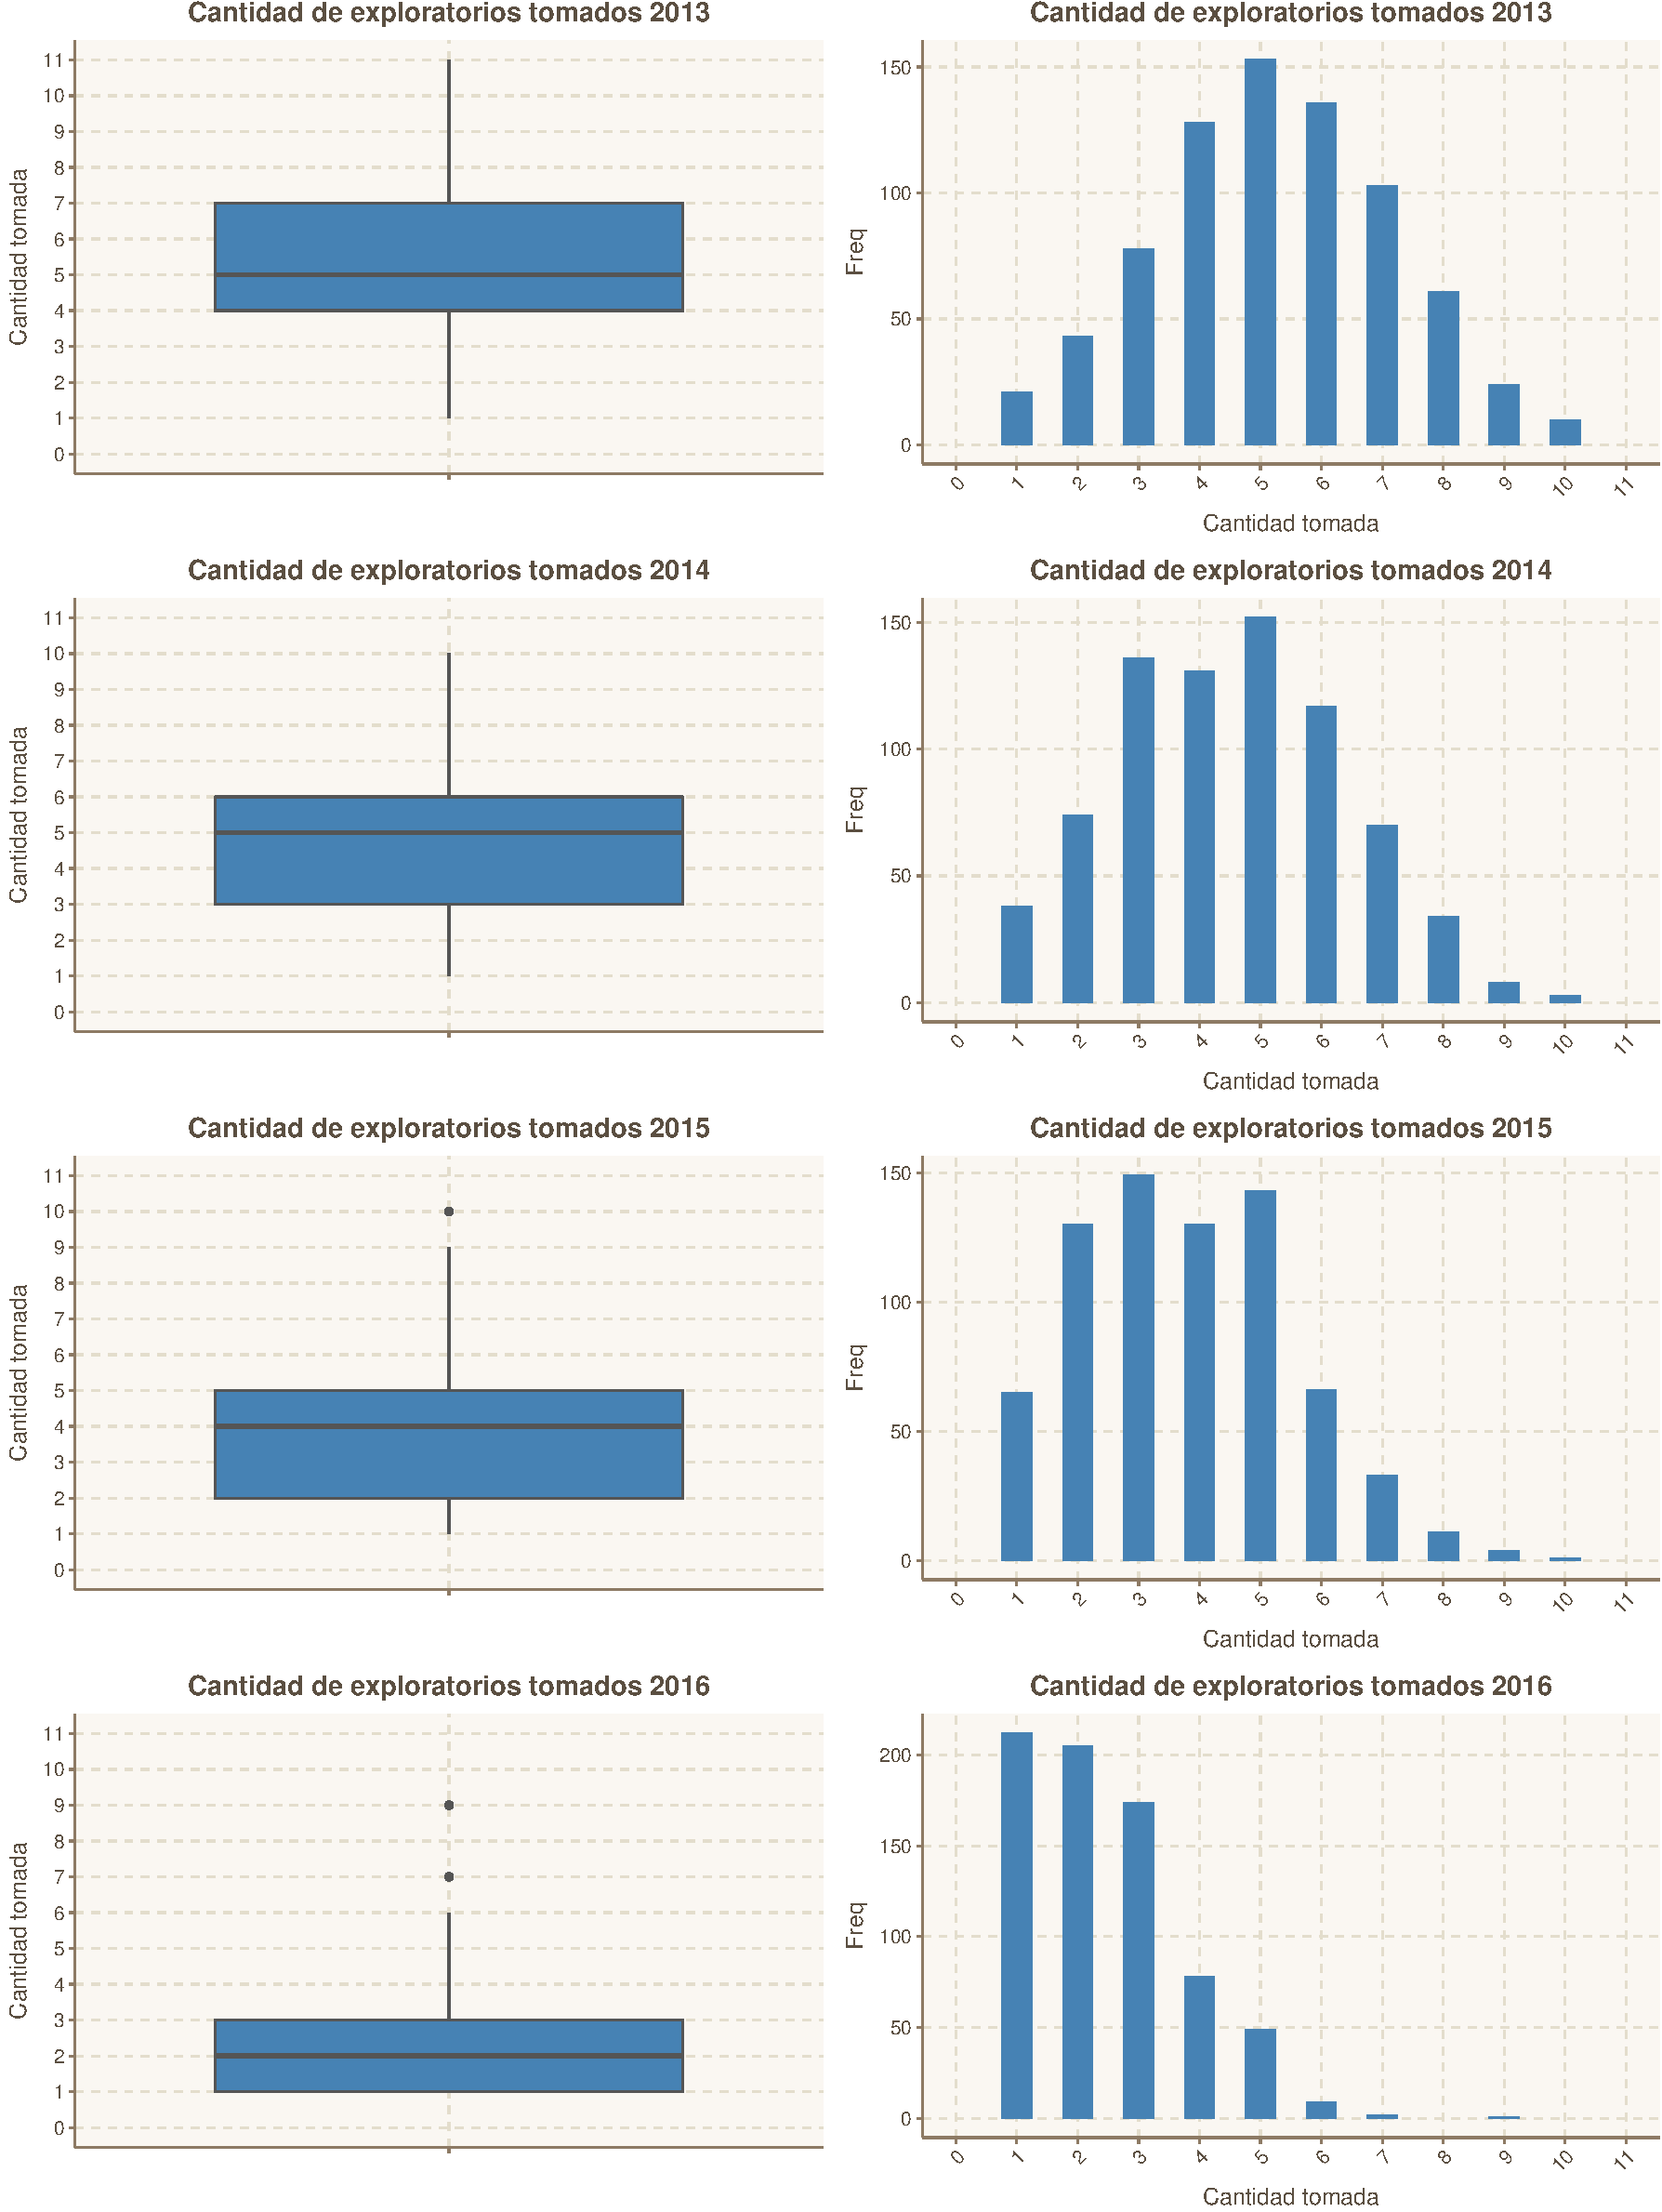
\includegraphics{Figs/plot1-1} \end{center}

\newline

Mismos gráficos pero ahora usando los datos concatenados

\begin{verbatim}
##    Min. 1st Qu.  Median    Mean 3rd Qu.    Max. 
##   1.000   2.000   4.000   4.021   5.000  11.000
\end{verbatim}

\begin{center}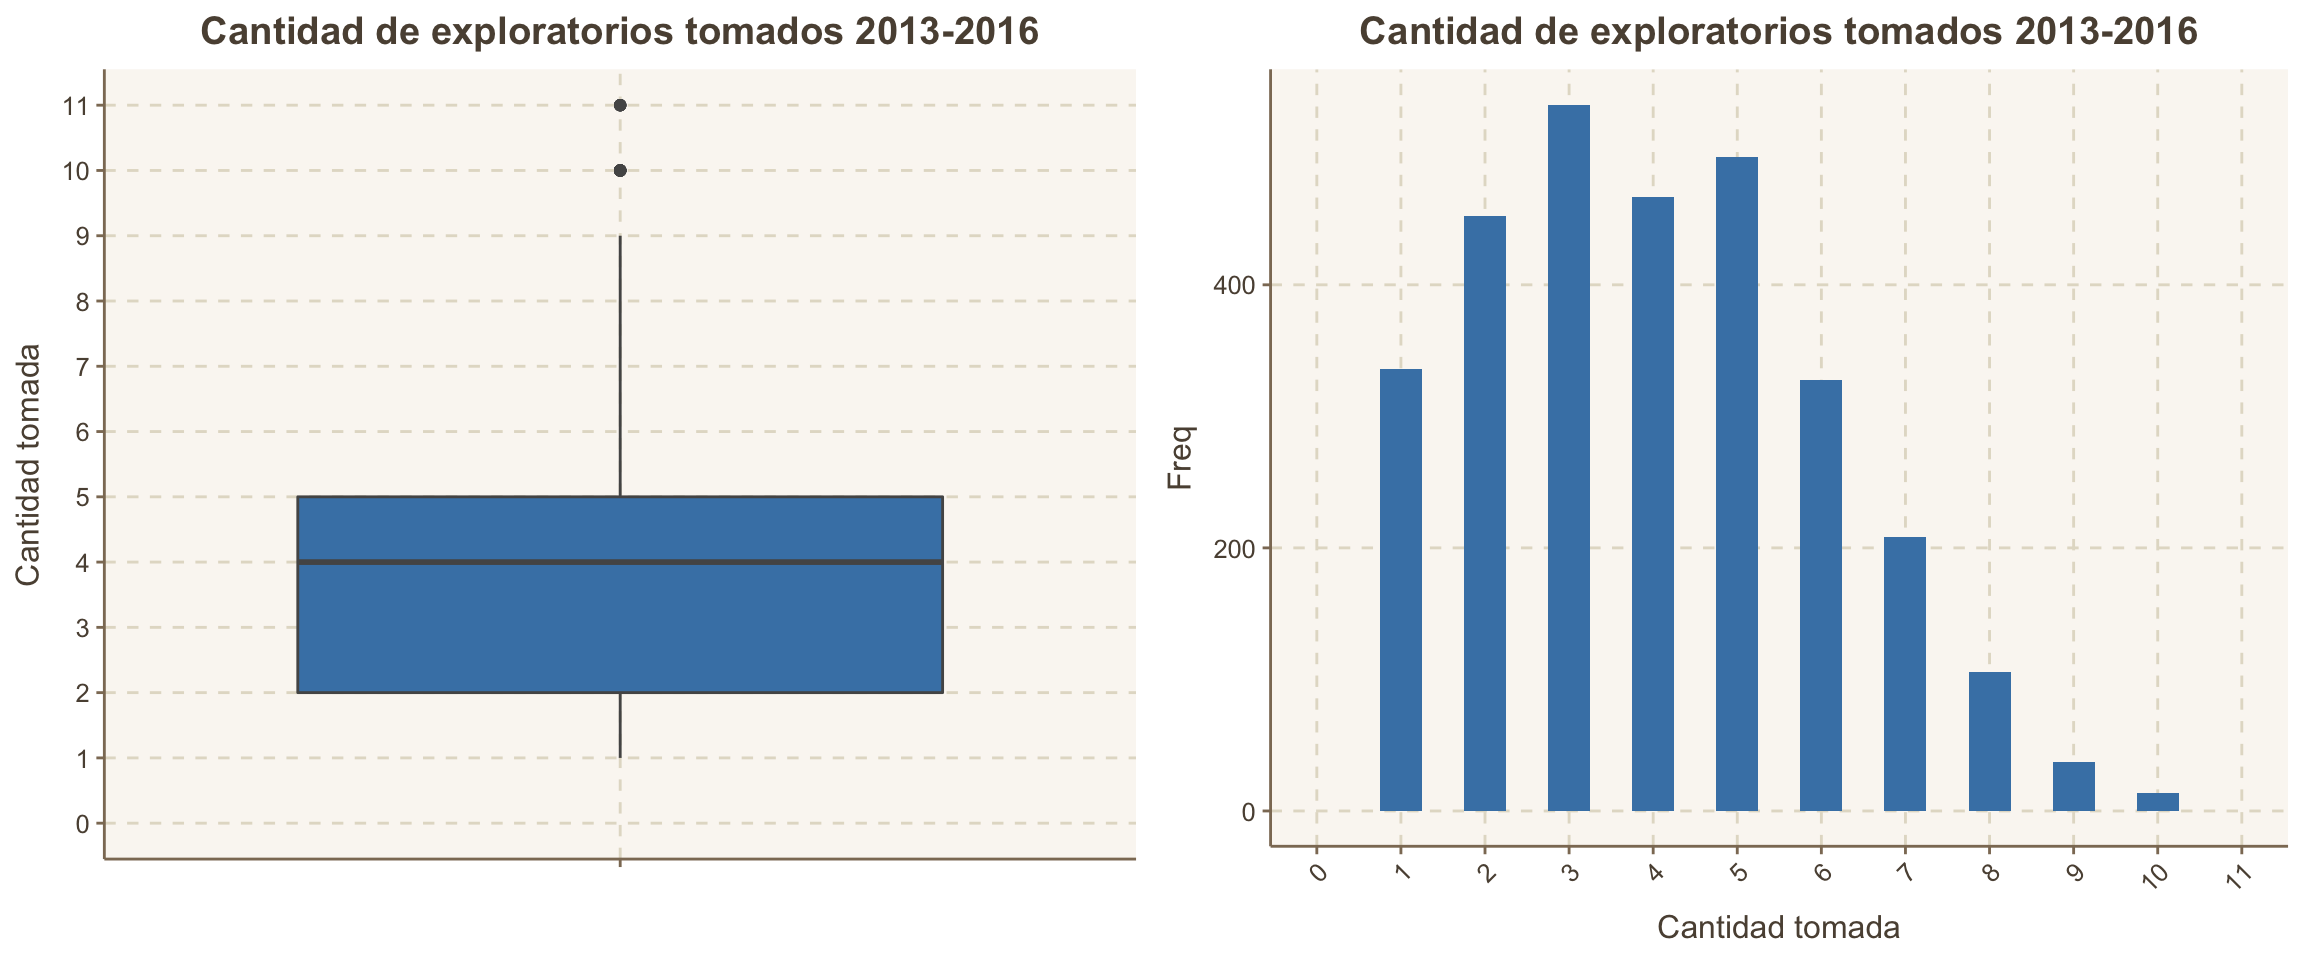
\includegraphics{Figs/unnamed-chunk-2-1} \end{center}


\end{document}
